\documentclass[pdflatex,sn-mathphys-num,iicol]{sn-jnl}

\usepackage[T1]{fontenc}
\usepackage{amsmath,amssymb}
\usepackage{algorithm}
\usepackage{algpseudocode}
\algrenewcommand\algorithmicrequire{\textbf{Input:}}
\algrenewcommand\algorithmicensure{\textbf{Output:}}
\usepackage{booktabs}
\usepackage{placeins}
\usepackage{array}
\usepackage{graphicx}
\usepackage{tikz}
\usepackage{pgfplots}
\pgfplotsset{compat=1.17}
\usetikzlibrary{arrows.meta,calc,positioning,patterns}
\hypersetup{hypertexnames=false}
\renewcommand{\topfraction}{0.9}
\renewcommand{\bottomfraction}{0.8}
\renewcommand{\textfraction}{0.07}
\renewcommand{\floatpagefraction}{0.8}
\renewcommand{\dbltopfraction}{0.9}
\renewcommand{\dblfloatpagefraction}{0.8}
\setcounter{topnumber}{3}
\setcounter{bottomnumber}{2}
\setcounter{totalnumber}{5}
\setcounter{dbltopnumber}{3}
\setlength{\floatsep}{12pt plus 3pt minus 2pt}
\setlength{\textfloatsep}{12pt plus 3pt minus 2pt}
\setlength{\dblfloatsep}{12pt plus 3pt minus 2pt}
\setlength{\dbltextfloatsep}{12pt plus 3pt minus 2pt}
\newcommand{\ci}[3]{\begin{tabular}[c]{@{}c@{}}$#1$\\{}[$#2$, $#3$]\end{tabular}}
\newcommand{\cib}[3]{{\boldmath\ci{#1}{#2}{#3}}}
\newcommand{\cit}[3]{\begin{tabular}[t]{@{}c@{}}$#1$\\{}[$#2$, $#3$]\end{tabular}}
\newcommand{\cibt}[3]{{\boldmath\cit{#1}{#2}{#3}}}
\newcommand{\scl}{SCL}
\newcommand{\aob}{AOB}
\newcommand{\twol}[2]{\begin{tabular}[c]{@{}l@{}}#1\\#2\end{tabular}}

\makeatletter
\def\email#1{\global\advance\emailcnt by 1\relax
\if@corauemail
  \ifx\corrauthemail\@empty\g@addto@macro\corrauthemail{\textcolor{blue}{#1}}%
  \else\g@addto@macro\corrauthemail{;\ \textcolor{blue}{#1}}\fi
\else
  \ifx\authemail\@empty\g@addto@macro\authemail{\textcolor{blue}{#1}}%
  \else\g@addto@macro\authemail{;\ \textcolor{blue}{#1}}\fi
\fi}
\makeatother

\makeatletter\setlength{\@fptop}{0pt}\setlength{\@dblfptop}{0pt}\makeatother
\begin{document}

\title[Self-Calibrating Control Layer for Multi-Object Trackers]{Training-Free Self-Calibrating Control Layer for Heterogeneous Multi-Object Trackers}

\abstract{Multi-object trackers use fixed score thresholds tuned for one detector. When the detector is replaced, retrained, or compressed, its confidence scores shift, the thresholds no longer fit, and nothing in the system detects the mismatch. This paper proposes a training-free self-calibrating control layer (\scl{}) placed between an unchanged detector and an unchanged tracker. It splits the logits of recent detection scores twice with Otsu's method and classifies the score stream as clean or noisy, without labels or future frames. Its novelty is selective, host-aware adaptation: on clean scores it keeps the tracker's own scores and thresholds, and only on noisy scores does it select and rescore the detections and set the thresholds, expressed through four published settings of the tracker, so one frozen configuration serves single-stage and two-stage trackers alike. The frozen layer was tested on seven published trackers, four detection sources, and three datasets; gains are relative to the tracker alone. Under detector change, two trackers that failed completely with halved scores recovered at least 97\% of their original higher order tracking accuracy (HOTA), and with a mismatched RT-DETR-L detector the multiple object tracking accuracy (MOTA) of ByteTrack and BoT-SORT rose by 12.6\% and 16.3\% with 43\% and 47\% fewer identity switches. Across trackers, HOTA rose for PD-SORT, which was not seen during design, while four well-matched trackers stayed within 0.1\%. \scl{} adds 2.95 ms per frame on an ordinary processor, so a detector can be updated without retuning the tracker.}


\keywords{multi-object tracking, tracking by detection, detector confidence calibration, online adaptation, Otsu thresholding, real-time image processing}

\maketitle

\section{Introduction}\label{sec:intro}

Multi-object tracking (MOT) finds every object of interest in a video and gives each one an
identity number (ID) that stays the same over time. It is used in surveillance, driving, and drone
systems \cite{zhu2022visdrone}, where results are needed with little delay. Most
MOT systems follow the tracking-by-detection design \cite{adzemovic2026survey}: in each frame, a
detector returns candidate boxes with confidence scores, and a tracker links them into tracks, one
per object \cite{bewley2016sort,zhang2022bytetrack,cao2023ocsort}. The tracker uses a box only if
its score passes a fixed threshold. A two-stage tracker, such as ByteTrack, also uses lower-score
boxes in a second step to continue unmatched tracks \cite{zhang2022bytetrack}; a single-stage
tracker, such as OC-SORT, ignores every box below one threshold \cite{cao2023ocsort}.

In real systems the detector is often replaced, retrained, or compressed, while the tracker keeps
the thresholds that its authors set for another detector. Detector scores are not calibrated across
models and conditions \cite{kuppers2020detcalib}, so a new detector usually gives scores on a
different scale, and nothing in the system notices. The effect can be large: halving the scores of
a published detector reduces two well-known trackers to 0 higher order tracking accuracy (HOTA)
\cite{luiten2021hota}, because no detection passes their thresholds (Sect.~\ref{sec:shift}). For example, ByteTrack in
its official setting starts a track only from a box with a score of at least 0.7; a car that the
original detector scored 0.9 now gets 0.45, so ByteTrack never starts a track, and its HOTA falls
from 67.70 to 0. \scl{} finds from the scores themselves that the confident group now begins
lower and lets it reach the tracker again, and ByteTrack reaches 66.17 HOTA again, with no labels and no change to its code.
Retuning every tracker for every detector needs labels, which a working system usually does not
have. Adaptive-threshold methods are each built into one tracker
\cite{ma2023adaptivebytetrack,shim2024adaptrack,act2026adaptive}, score calibration needs
labelled data \cite{kuppers2020detcalib}, and adaptive inference methods learn their settings for
one model \cite{han2022dynamic}.

This paper presents a self-calibrating control layer (\scl{}) that sits between a detector and a
tracker that are both kept fixed (frozen): their code, weights, and stored settings are not
changed. We call the tracker that \scl{} serves the \emph{host}. The novelty of \scl{} is
\emph{selective, host-aware adaptation}. It is selective because it first decides, from the
detector scores alone and without labels, whether the scores of the stream fit the host at all:
when most higher scores of recent frames form a clearly confident group, the stream is clean, and
the host keeps its scores and, unless they would reject the confident group, its thresholds. Only
when many scores are uncertain does \scl{} take control: it chooses which candidates reach the
host, gives them new scores, and sets the host's thresholds for the frame. It is host-aware because
every action is expressed in the host's own terms: four published settings of the host, the host
contract (Sect.~\ref{sec:contract}), tell the layer where the host's thresholds lie and whether it
has a low-score step, so the same frozen rules serve single-stage and two-stage trackers.

With halved detector scores, \scl{} restored two trackers from 0 to about 66 HOTA; with other
detectors, it raised the multiple object tracking accuracy (MOTA) of two-stage trackers by up to
24.7 points and cut their identity switches by 43\% to 56\%, while well-matched strong trackers
stayed within 0.06 HOTA points of their own accuracy.

The main contributions are:
\begin{enumerate}
\item \emph{Selective adaptation.} A label-free, causal test of detector--tracker compatibility:
      nested Otsu splits of recent logits and a whole-stream majority rule decide whether to act,
      so a well-matched system is left as it is and a mismatched one is corrected
      (Sects.~\ref{sec:calib}--\ref{sec:choice}).
\item \emph{Host-aware adaptation.} A host contract of four published values through which one
      fixed configuration sets the thresholds, scores, and matching tolerance of unchanged
      single-stage and two-stage trackers, with a track-guided recovery of weak detections for
      trackers that lack a low-score step (Sects.~\ref{sec:rescue}--\ref{sec:contract}).
\item \emph{Evidence for compatibility.} An evaluation of one frozen configuration on seven
      trackers, four detection sources, and three datasets, with paired bootstrap intervals,
      comparisons with adaptive thresholds and the published ACT method, a component ablation and a
      parameter sensitivity analysis (Sect.~\ref{sec:results}), the recorded development path
      (Sect.~\ref{sec:development}), and a cost of about 3 ms per frame on an ordinary processor
      (central processing unit, CPU) (Sect.~\ref{sec:discussion}).
\end{enumerate}

Section~\ref{sec:related} covers the data, metrics, and related work;
Sections~\ref{sec:method} and~\ref{sec:development} present \scl{} and its development;
Section~\ref{sec:results} gives the results; and Sections~\ref{sec:discussion}
and~\ref{sec:conclusion} discuss and conclude.

\section{Background and Related Work}\label{sec:related}

\subsection{Datasets}\label{sec:data}
Three public datasets are used. \emph{MOT17} \cite{milan2016mot16} contains 14 sequences of
people filmed with static and moving cameras. As is common, the second half of each of the seven
training sequences, called val-half (2,652 frames), is used for evaluation \cite{zhang2022bytetrack},
with the published YOLOX-X detections \cite{ge2021yolox} at the two published emission floors, the
lowest scores emitted, of 0.01 and 0.1. To study score changes directly, these scores were also
changed before the tracker by four transforms that keep their order: cubing ($s^3$), halving
($0.5\,s$), and logit temperatures $T=2$ and $T=0.5$, which divide the logit (log-odds, Sect.~\ref{sec:problem}) of each score by $T$.
\emph{KITTI tracking} \cite{geiger2012kitti} has 21 training sequences (8,008 frames) recorded from
a car and is scored on cars and pedestrians; here the trackers run with two other detectors,
YOLOv8n \cite{jocher2023yolov8} and RT-DETR-L \cite{zhao2024rtdetr}, and keep thresholds that were
set for other detectors. \emph{UAVDT} \cite{du2018uavdt} contains drone videos of vehicles; its 20
test sequences (16,592 frames) are used with ByteTrack, YOLOv8n, and RT-DETR-L.

MOT17 with four trackers, KITTI, and the score transforms were development data, looked at while
\scl{} was designed. Two predeclared external trackers, PD-SORT and Hybrid-SORT, were chosen in
advance and run once with the frozen configuration on the detections released by their authors on
MOT17 val-half. The held-out UAVDT test split was also run once, after a written plan. Each
external host was checked against its authors' number: EXACT within 0.2 HOTA points, CLOSE within
1.0.

\subsection{Evaluation metrics}\label{sec:metrics}
HOTA \cite{luiten2021hota}, the main metric, balances finding the objects and keeping their
identities,
\begin{equation}
\mathrm{HOTA}=\frac{1}{19}\sum_{\alpha}\sqrt{\mathrm{DetA}_\alpha\,\mathrm{AssA}_\alpha},
\label{eq:hota}
\end{equation}
where $\mathrm{DetA}_\alpha$ and $\mathrm{AssA}_\alpha$ are the detection and association accuracy
at the localization threshold $\alpha=0.05,0.10,\dots,0.95$. MOTA \cite{bernardin2008clear} and
IDF1 \cite{ristani2016idf1} are
\begin{align}
\mathrm{MOTA}&=1-\frac{\mathrm{FN}+\mathrm{FP}+\mathrm{IDS}}{\mathrm{GT}},\label{eq:mota}\\
\mathrm{IDF1}&=\frac{2\,\mathrm{IDTP}}{2\,\mathrm{IDTP}+\mathrm{IDFP}+\mathrm{IDFN}},\label{eq:idf1}
\end{align}
where FN are missed objects (false negatives), FP false positives, IDS identity switches (an
object's ID changes), and GT the number of ground-truth boxes; IDTP, IDFP, and IDFN count boxes
after each ground-truth track is matched to at most one output track. All metrics are computed
with TrackEval (commit 12c8791) and the official ground truth \cite{dendorfer2021motchallenge};
KITTI HOTA is averaged over cars and pedestrians, and on UAVDT all vehicles form one class and
predictions in ignored regions are removed. HOTA, MOTA, and IDF1 are in percent, and differences
in points.

All comparisons are paired: each tracker runs alone and with \scl{} on the same sequences and
detections. Paired bootstrap resampling of whole sequences \cite{efron1993bootstrap}, 10,000 times
with seed 42, gives a 95\% interval (2.5--97.5 percentiles) for each difference, which is called
significant when its interval does not include zero.

\subsection{Related work}\label{sec:survey}
\emph{Tracking by detection.}\label{sec:hosts} SORT matches Kalman-filter predictions to new
detections by their overlap \cite{bewley2016sort}; ByteTrack added a second step that uses
low-score detections to continue tracks \cite{zhang2022bytetrack}; OC-SORT uses one score
threshold \cite{cao2023ocsort}. Their thresholds were tuned for one detector, usually YOLOX
\cite{ge2021yolox}. Many recent trackers improve association with trained or domain-specific
parts \cite{li2024fdbtrack,bao2024graphmatching,zhang2025sinkhorn,ding2025remot,liang2024motiontrack,sun2026bsr},
which change or retrain the tracker; \scl{} keeps both the tracker and the detector unchanged.
Seven published trackers serve as hosts in this study, each with the authors' code and published
configuration: ByteTrack, BoT-SORT \cite{aharon2022botsort}, OC-SORT, SparseTrack
\cite{liu2025sparsetrack}, BoostTrack \cite{stanojevic2024boosttrack}, PD-SORT
\cite{wang2025pdsort}, and Hybrid-SORT \cite{yang2024hybridsort}. ByteTrack is used with the
thresholds that its authors used on MOT17 (official setting) and with the defaults of the
Ultralytics library, which also provides BoT-SORT (library setting).

\emph{Adaptive thresholds.} Adaptive ByteTrack sets ByteTrack's threshold from each frame
\cite{ma2023adaptivebytetrack}, AdapTrack adapts its matching thresholds \cite{shim2024adaptrack},
and ACT sets the high and low thresholds from the first quartile and the number of the current
scores \cite{act2026adaptive}. ConfTrack weights the Kalman update and the matching cost by the
score \cite{jung2024conftrack}, and PlugTrack blends motion predictors with a trained network
\cite{kim2026plugtrack}.

\emph{Comparison.} Table~\ref{tab:compare} compares \scl{} with the adaptive-thresholding and
score-calibration methods. The adaptive-thresholding methods act in every frame, read only the
current frame or each box, and are built into one tracker; calibration acts on every score and
needs labelled data. \scl{} differs in three ways. It is selective: it first decides, from the
scores of past frames, whether to act at all, and leaves a well-matched tracker as it is. It is
host-aware: it reads the tracker's published settings and serves several unchanged single-stage
and two-stage trackers through them. And it needs neither labels nor trained parts; its new scores
encode decisions for the tracker's thresholds rather than calibrated probabilities
(Sect.~\ref{sec:choice}). It is also tested as one frozen configuration under score changes and on
external systems, and against ACT on the same detections (Sect.~\ref{sec:baselines}).

\begin{table*}[!tp]
\caption{\scl{} compared with adaptive-thresholding and score-calibration methods. ReID:
re-identification network.}
\label{tab:compare}
\centering\footnotesize
\setlength{\tabcolsep}{3pt}
\begin{tabular}{@{}>{\raggedright\arraybackslash}p{23mm}>{\raggedright\arraybackslash}p{28mm}>{\raggedright\arraybackslash}p{28mm}>{\raggedright\arraybackslash}p{19mm}>{\raggedright\arraybackslash}p{24mm}>{\raggedright\arraybackslash}p{25mm}@{}}
\toprule
Method & What is adapted & Information used & Labels or trained parts & When it acts & Where it works\\
\midrule
\multicolumn{6}{@{}l}{\textit{Adaptive thresholding}}\\
Adaptive ByteTrack \cite{ma2023adaptivebytetrack} & high/low score split & scores of the current frame & none & every frame & inside ByteTrack\\
AdapTrack \cite{shim2024adaptrack} & matching thresholds & current frame & ReID network & every frame & its own tracker\\
ACT \cite{act2026adaptive} & high and low thresholds, chosen from preset levels & first quartile and number of the current scores & none & every frame & inside the tracker\\
ConfTrack \cite{jung2024conftrack} & Kalman update and matching cost & score of each box & ReID network & every box & its own tracker\\
\addlinespace[3pt]
\multicolumn{6}{@{}l}{\textit{Score calibration}}\\
K{\"u}ppers et al.\ \cite{kuppers2020detcalib} & detector scores, mapped to probabilities & labelled data & calibration map & every score & detector output\\
\addlinespace[3pt]
\multicolumn{6}{@{}l}{\textit{This paper}}\\
\scl{} & candidates, scores, thresholds, matching tolerance & logits of past frames; host contract & none & only when the scores are noisy (clean: thresholds capped) & between a detector and unchanged trackers\\
\bottomrule
\end{tabular}
\end{table*}


\emph{Score calibration and adaptive inference.} Detector families such as YOLOX, YOLOv8, and RT-DETR give different score distributions,
and calibration methods learn a mapping from labelled data \cite{kuppers2020detcalib}. Otsu's
method picks, without labels, the threshold that best splits a histogram into two groups
\cite{otsu1979}; \scl{} applies it to the logits of recent scores. Dynamic networks learn their
settings for each model \cite{han2022dynamic}, and a separate controller, AC-MOT (submitted), sets the detector operating point from
image and track cues. \scl{} instead reads the scores and acts on the tracker's input and
thresholds.

\section{Proposed SCL Framework}\label{sec:method}

\scl{} is a small, rule-based layer that runs once per frame between a frozen detector and a
frozen tracker, the host, and changes neither. Figure~\ref{fig:arch} shows its five steps for
frame $t$, and this section follows them in order. The top row is the path of the detections:
candidate selection (Step~3) keeps, drops, or rescores them, weak detection recovery (Step~4)
passes weak boxes that continue tracks, and the tracker matches them as usual. The bottom row sets
this path: logit partitioning (Step~1) groups the recent scores, stream classification (Step~2)
decides whether they are clean or noisy, the host contract gives the tracker's published settings,
and the motion-adaptive tolerance (Step~5) sets how loosely the tracker matches boxes.

\begin{figure*}[t]
\centering
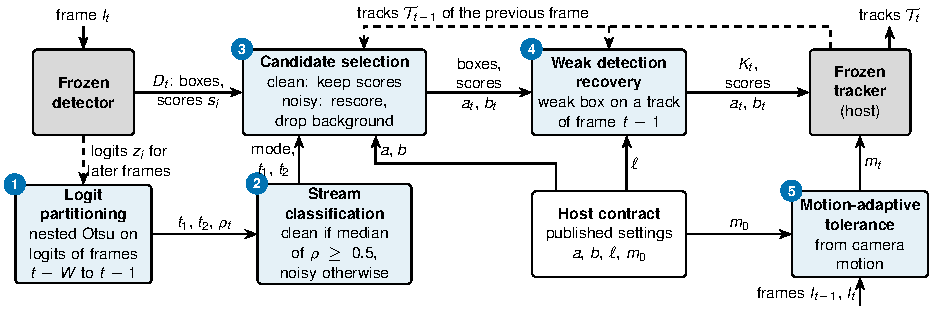
\includegraphics{Fig1.pdf}
\caption{\scl{} between a frozen detector and a frozen tracker (the host), for frame $t$. Each
arrow is labelled with the data it carries; dashed arrows carry data kept from earlier frames.
Steps 1--5 are described in Sects.~\ref{sec:calib}--\ref{sec:motion}, and the host contract in
Sect.~\ref{sec:contract}}
\label{fig:arch}
\end{figure*}

\subsection{Inputs and outputs of SCL}\label{sec:problem}
In each frame $t$, the detector gives candidates $D_t=\{(\mathbf{x}_i,s_i,c_i)\}$, each with a box
$\mathbf{x}_i$, a score $s_i\in(0,1)$, and a class $c_i$. The layer works on the logit
\begin{equation}
z_i=\log\frac{s_i}{1-s_i},
\label{eq:logit}
\end{equation}
the log-odds transformation of the confidence score. It maps a score between 0 and 1 to an
unbounded scale and keeps the order of the scores: a score of 0.5 gives $z_i=0$, 0.9 about $2.2$,
and 0.1 about $-2.2$. The logistic function $\sigma(z)=1/(1+e^{-z})$ turns a logit back into a
score. The layer uses logits for two reasons. Detector scores crowd near 0 and 1, where small
differences in score are large differences in confidence; the logit spreads these regions out, so
the splits of Step~1 separate the groups more clearly. And a common change of a detector's scores,
a change of temperature, divides all logits by the same number; the splits follow this stretch,
and each group keeps the same candidates. The host gives its contract $h=(a,b,\ell,m_0)$: the score $a$ needed to match a track, the
score $b$ needed to start one, the lowest score $\ell$ it uses, and its matching tolerance $m_0$,
one minus the smallest intersection over union (IoU) of two boxes that counts as a match. A
single-stage tracker has $\ell=\min(a,b)$, a two-stage tracker $\ell<\min(a,b)$. In every frame
the layer returns
\begin{equation}
\left(K_t,\tilde{s},a_t,b_t,m_t\right)=
\mathcal{L}\left(Z_{<t},D_t,\mathcal{T}_{t-1},g_t;\,h\right):
\label{eq:layer}
\end{equation}
the candidates $K_t$ for the tracker, their scores, and its thresholds and tolerance (the arrows
into the tracker in Fig.~\ref{fig:arch}), from the logits $Z_{<t}$ of earlier frames, the tracks
$\mathcal{T}_{t-1}$, and the camera motion $g_t$ between the frames $I_{t-1}$ and $I_t$; no future
frame is used.

\subsection{Otsu-Based Logit Partitioning and Confidence Estimation}\label{sec:calib}
\emph{Step 1 in Fig.~\ref{fig:arch}. Input:} the logits $Z_t^W$ of the candidates of the last $W=10$ frames. \emph{Output:} the
splits $t_1$, $t_2$ and the confident share $\rho_t$.

The logits are split twice with Otsu's method \cite{otsu1979}, which picks, from the data alone
and without labels or tuning, the threshold that best separates a set of values into two groups;
applied twice, it gives the three groups that one threshold cannot. The first split, $t_1$,
separates background (low logits) from foreground; the second, $t_2$, found on the foreground only,
divides it into uncertain and confident candidates. The share of confident candidates in the
foreground,
\begin{equation}
\rho_t=\frac{\left|\{z\in Z_t^W: z\ge t_2\}\right|}{\left|\{z\in Z_t^W: z\ge t_1\}\right|},
\label{eq:rho}
\end{equation}
describes the shape of the score distribution. For example, for the scores
0.02, 0.03, 0.05, 0.4, 0.5, 0.9, and 0.95 (logits $-3.9$, $-3.5$, $-2.9$, $-0.4$, 0, 2.2, and 2.9),
the first split separates the three lowest scores as background, and the second divides the other
four into 0.4 and 0.5 (uncertain) and 0.9 and 0.95 (confident), so $\rho_t=2/4=0.5$. Figure~\ref{fig:groups} shows the groups for a
clean and a noisy stream. When a detector emits very few low scores, the first split falls inside
the objects; since clutter usually gives more candidates than the objects do, a window with fewer
candidates below $t_1$ than above it counts as clean, $\rho_t=1$ (background check).

\begin{figure}[t]
\centering
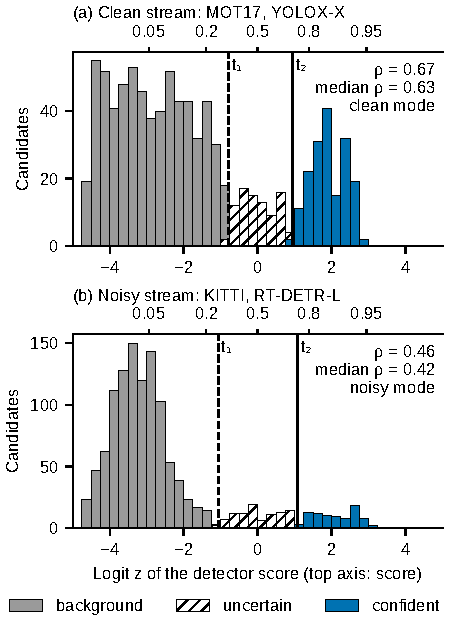
\includegraphics{Fig2.pdf}
\caption{What the layer sees: the logits of the candidates of the last 10 frames, just before its
decision for frame 101, with the Otsu splits $t_1$ (dashed line) and $t_2$ (solid line). Plain
light bars: background; hatched bars: uncertain; plain dark bars: confident. The top axis gives the
matching detector score. (a) MOT17-02 with YOLOX-X: most foreground candidates are confident, and
the stream is clean. (b) KITTI 0001 with RT-DETR-L: many are uncertain, and the stream is noisy.
Values of the frozen layer in the runs of Sect.~\ref{sec:results}}
\label{fig:groups}
\end{figure}

\subsection{Median-Based Detection Stream Classification}\label{sec:regimes}
\emph{Step 2 in Fig.~\ref{fig:arch}. Input:} the values $\rho$ of all frames so far. \emph{Output:} the mode of frame $t$.

The mode describes the distribution of the scores, not whether a single detection is correct. The
stream is clean at frame $t$ if the median of all $\rho$ values so far is at least one half, a
majority rule, and noisy otherwise; before the first valid split it is cold.

\emph{Mode stability and adaptation delay.} The whole-stream median trades speed for stability. A
short run of low scores, such as a few frames of blur or occlusion, cannot change the mode, so the
layer does not switch modes in the middle of a stream; during development this rule raised the
HOTA of ByteTrack and OC-SORT (Sect.~\ref{sec:steps}). The cost is a delay after a lasting change
of the detector within one stream: a stream that was clean for $N$ frames turns noisy only after
more than $N$ noisy frames, because only then do they form the majority of the $\rho$ values. Two
parts of the layer do not wait. The splits use only the last $W$ frames, so the groups, and in
the clean mode the thresholds of Step~3, follow a new score scale within $W$ frames, and the
recovery of Step~4 works in both modes; only the rescoring of the noisy mode waits for the mode. A
median over the last $K$ frames bounds the delay to about $K/2$ frames;
Sect.~\ref{sec:ablation} tests $K=100$ and $K=300$.

\subsection{Mode-Adaptive Detection Candidate Selection and Threshold Adjustment}\label{sec:choice}
\emph{Step 3 in Fig.~\ref{fig:arch}. Input:} $D_t$, the mode, $t_1$, $t_2$, the thresholds $a$, $b$, and the tracks
$\mathcal{T}_{t-1}$. \emph{Output:} the kept boxes, their scores, and the thresholds $a_t$, $b_t$.

\emph{Cold and clean modes.} The tracker keeps its own thresholds and scores, and only cross-class
duplicates are removed. In the clean mode, a threshold so high that it would reject the confident
group is lowered to the score $\sigma(t_2)$ at which that group begins:
\begin{equation}
a_t=\min\!\left(a,\sigma(t_2)\right),\qquad b_t=\min\!\left(b,\sigma(t_2)\right).
\label{eq:clean}
\end{equation}
The clean mode is thus a minimal intervention rather than a plain pass-through: the scores are
kept, and the output equals that of the host alone whenever the confident group lies above the
host's thresholds and no rescue applies, as for BoostTrack, ByteTrack at floor 0.1, and Hybrid-SORT
on MOT17 (Sect.~\ref{sec:results}). When the scores are halved, for example, no score is above 0.5,
and ByteTrack in its official setting ($a=0.6$, $b=0.7$) never starts a track; the splits move with
the halved scores, so Eq.~\eqref{eq:clean} lets the confident candidates reach it again.

\emph{Noisy mode.} Background candidates ($z<t_1$) are dropped. Each remaining score is
replaced by its mid-rank $u_i\in(0,1)$ among the scores of a remap memory, which stores the scores
kept in the first frame and in every 10th frame, the last 20 of them (tied scores share their
average rank, and before the first sample the current frame is used),
\begin{equation}
\tilde{s}_i=
\begin{cases}
0.5+0.5\,u_i, & z_i\ge t_2,\\
0.1+0.4\,u_i, & t_1\le z_i<t_2,
\end{cases}
\label{eq:remap}
\end{equation}
and both thresholds are set to $a_t=b_t=0.5$. Confident candidates ($z\ge t_2$) then get scores above 0.5
and may start and continue tracks, and uncertain ones ($t_1\le z<t_2$) get scores below 0.5 and may
only continue tracks through a tracker's low-score step. A weaker
candidate that overlaps a stronger one with IoU above one half is removed, unless a different track
of the previous frame claims it, which keeps people who stand close together in a crowd.

\emph{Score remapping is not probability calibration.} Formal calibration learns, from labelled
data, a map from a score to the probability that the detection is correct \cite{kuppers2020detcalib}.
The remap of Eq.~\eqref{eq:remap} needs no labels and estimates no probability. It keeps the order
of the scores within each group and places the groups in fixed ranges, so that the tracker's own
thresholds read the decision of the layer: a score above 0.5 means ``may start a track'', a score
between 0.1 and 0.5 ``may only continue one''. A remapped score of 0.8 therefore says that the
candidate ranks high among recent confident candidates, not that it is correct with probability
0.8. Because only ranks are used, the remap itself is unchanged by any order-preserving change of
the detector's scores, whereas a learned calibration map would have to be learned again.

\subsection{Track-Guided Weak Detection Recovery}\label{sec:rescue}
\emph{Step 4 in Fig.~\ref{fig:arch}. Input:} the output of Step~3, the tracks $\mathcal{T}_{t-1}$, and $\ell$. \emph{Output:}
$K_t$, their scores, and $a_t$, $b_t$ for the tracker.

A track can be lost when its object gets low scores for a few frames, above all in single-stage
trackers, which have no low-score step. The rescue passes such a candidate, with its score raised
just above the lowest threshold of the frame ($\ell$ for a two-stage tracker, the lower of $a_t$
and $b_t$ for a single-stage one), when it is in the foreground (or, for a single-stage tracker,
when there is no background group), overlaps a track of the previous frame with IoU of at least
one half, no other usable candidate covers that track, and the tracker could not see it otherwise.
It thus gives single-stage trackers the continuation step they lack. The rescue only makes the box
visible; the tracker itself still decides, with its own matching, whether and to which track it is
assigned.

\subsection{Camera Motion-Adaptive Matching Tolerance}\label{sec:motion}
\emph{Step 5 in Fig.~\ref{fig:arch}. Input:} the frames $I_{t-1}$, $I_t$ and the tolerance $m_0$. \emph{Output:} the tolerance
$m_t$ of frame $t$.

In noisy frames, the matching tolerance grows with camera motion, because fast motion moves boxes
far from their tracks; otherwise $m_t=m_0$. The motion $g_t$ is the shift between consecutive
grayscale frames at quarter resolution, found by phase correlation \cite{reddy1996phasecorr}, and
$r_t$ is its ratio to its median over the last 100 frames ($r_t=1$ during a warm-up of 5 frames or
if this median is zero):
\begin{equation}
m_t=\min\!\left(0.95,\;1-\frac{1-m_0}{\max(1,r_t)}\right).
\label{eq:motion}
\end{equation}
With $m_0=0.8$ and twice the usual motion, a match needs an IoU of 0.1 instead of 0.2.

\subsection{SCL Integration with Existing Trackers}\label{sec:contract}
Table~\ref{tab:contracts} lists the contracts; each value is taken from the tracker's published
configuration, and none is fitted. For each tracker family, a small adapter links the layer to the
tracker block of Fig.~\ref{fig:arch}: it writes the layer's candidates, scores, thresholds, and
tolerance into the tracker's existing parameters before each update and then calls the tracker's
own update. The matching steps, motion model, track management, and any post-processing of the
authors run unchanged, so the host stays frozen: only the values of its thresholds are set for
each frame, and the rules are the same for every tracker.

\begin{table}[!tb]
\caption{Host contracts: the published settings of each tracker, as used by the layer: matching
(association) threshold $a$, birth threshold $b$, low threshold $\ell$, and match tolerance $m_0$.
For every tracker, the layer's decision is passed on as thresholds, candidates, and scores.}
\label{tab:contracts}
\centering\footnotesize
\setlength{\tabcolsep}{4pt}
\begin{tabular}{@{}>{\raggedright\arraybackslash}p{27mm}lcccc@{}}
\toprule
Tracker (setting) & Type & $a$ & $b$ & $\ell$ & $m_0$\\
\midrule
ByteTrack (official MOT17) & two-stage & 0.6 & 0.7 & 0.1 & 0.8\\
ByteTrack (library default) & two-stage & 0.25 & 0.25 & 0.1 & 0.8\\
BoT-SORT (library default) & two-stage & 0.25 & 0.25 & 0.1 & 0.8\\
SparseTrack & two-stage & 0.6 & 0.7 & 0.1 & 0.85\\
BoostTrack & two-stage & 0.6 & 0.6 & 0.1 & 0.7\\
Hybrid-SORT & two-stage & 0.6 & 0.6 & 0.1 & 0.75\\
OC-SORT & single-stage & 0.6 & 0.6 & 0.6 & 0.7\\
PD-SORT & single-stage & 0.6 & 0.6 & 0.6 & 0.7\\
\bottomrule
\end{tabular}
\end{table}


\subsection{Fixed SCL Parameters}\label{sec:constants}
Table~\ref{tab:constants} lists all values of \scl{}. They were fixed before the external
evaluation, are the same for every tracker, detector, and dataset, and none was chosen by searching
over a range of values. They come from standard values (the IoU of 0.5 of MOT evaluation and the
common thresholds 0.5 and 0.1), from definitions, and from design choices kept fixed in all
development stages. Algorithm~\ref{alg:layer} gives Steps 1--5 for one frame.

\begin{table}[!tb]
\caption{Values of \scl{} and their source.}
\label{tab:constants}
\centering\footnotesize
\setlength{\tabcolsep}{3pt}
\begin{tabular}{@{}>{\raggedright\arraybackslash}p{19mm}>{\raggedright\arraybackslash}p{27mm}>{\raggedright\arraybackslash}p{25mm}@{}}
\toprule
Value & Setting & Source\\
\midrule
Window $W$ & 10 frames & design choice\\
Mode rule & clean if median $\rho\ge0.5$ & majority rule\\
Background check & $\rho=1$ if fewer below $t_1$ than above & rule: no background group\\
Noisy score ranges & $[0.5,1)$, $[0.1,0.5)$ & common thresholds\\
Noisy $a_t$, $b_t$ & 0.5 & common threshold\\
Remap memory & 20 frames, one every 10 & design choice\\
Duplicate, rescue IoU & 0.5 & MOT evaluation IoU\\
Rescued score & lowest threshold $+\,0.001$ & just above the threshold\\
Motion cue & phase correlation, quarter resolution & standard method \cite{reddy1996phasecorr}\\
Motion history & 100 frames, warm-up 5 & design choice\\
Tolerance cap & 0.95 & minimum overlap 0.05\\
\bottomrule
\end{tabular}
\end{table}


\begin{algorithm}[t]
\caption{\scl{} for frame $t$; the comments name the steps of Fig.~\ref{fig:arch}. The window
holds the logits of frames $t-W$ to $t-1$, so the decision for frame $t$ uses no future frame.}\label{alg:layer}
\begin{algorithmic}[1]
\Require candidates $D_t$, tracks $\mathcal{T}_{t-1}$, motion cue $g_t$, contract $(a,b,\ell,m_0)$, constants of Table~\ref{tab:constants}
\Ensure candidates $K_t$, scores $\tilde{s}$, thresholds $a_t,b_t$, tolerance $m_t$
\State $z_i\gets$ logit of $s_i$ for all $i$ \Comment{Eq.~\eqref{eq:logit}}
\If{no valid split exists} \Comment{e.g., first frame}
  \State mode $\gets$ cold; $(a_t,b_t)\gets(a,b)$
\Else
  \State $(t_1,t_2)\gets$ nested Otsu on the window \Comment{Step 1}
  \State $\rho_t\gets$ Eq.~\eqref{eq:rho} with the background check
  \State mode $\gets$ clean if $\mathrm{median}(\rho)\ge0.5$, else noisy \Comment{Step 2}
\EndIf
\If{mode is cold or clean} \Comment{Step 3}
  \State remove cross-class duplicates; keep raw scores
  \If{clean} set $(a_t,b_t)$ by Eq.~\eqref{eq:clean}
  \EndIf
\Else \Comment{noisy mode}
  \State remove duplicates with track context
  \State drop $z<t_1$; remap scores by Eq.~\eqref{eq:remap}
  \State $a_t\gets0.5$; $b_t\gets0.5$
\EndIf
\State rescue continuations (not cold) \Comment{Step 4}
\State $m_t\gets$ Eq.~\eqref{eq:motion} if noisy, else $m_0$ \Comment{Step 5}
\State pass $K_t$, $\tilde{s}$, $a_t$, $b_t$, $m_t$ to the tracker
\State add the logits left after duplicate removal to the window
\State add $g_t$ to the motion history
\State store the tracks of frame $t$ after the tracker update
\end{algorithmic}
\end{algorithm}

\section{SCL Development and Refinement}\label{sec:development}

\scl{} was developed in three stages on the development data of Sect.~\ref{sec:data}: a starting
point, design steps that each removed one cause found before them (Table~\ref{tab:ablation}), and a
freeze before any external test. The section reports this history as it was recorded at the time:
the steps, their order, and their numbers are those measured before the freeze, and later results
did not change them.

\begin{table*}[!tp]
\caption{Design steps from \aob{} to \scl{} on development
data (HOTA, \%), and versions that were tested and rejected. The floor of
ByteTrack and OC-SORT is given in parentheses.}
\label{tab:ablation}
\centering\footnotesize
\setlength{\tabcolsep}{4pt}
\begin{tabular}{@{}>{\raggedright\arraybackslash}p{25mm}>{\raggedright\arraybackslash}p{36mm}>{\raggedright\arraybackslash}p{62mm}@{}}
\toprule
Step & Change & Effect\\
\midrule
\aob{} emulated & always-noisy bands, overlap deduplication, rank remap & ByteTrack (0.1) 56.41 vs host 67.70; OC-SORT (0.1) 45.72 vs 66.44\\
+ mode gate & mode statistic, host-anchored clean mode, crowd-safe duplicates & SparseTrack 64.72 to 68.93 (host 68.88); BoostTrack 62.61 to 68.37 (host 68.49)\\
+ whole-stream mode & mode from all past frames & ByteTrack (0.1) 67.561 to 67.702; OC-SORT (0.1) 65.697 to 66.071\\
+ continuation rescue & foreground track-consistent rescue & OC-SORT (0.01) 66.405 to 66.619; OC-SORT (0.1) 66.071 to 66.469\\
+ background check = \scl{} & no background mode gives no evidence against the host & ByteTrack/BoostTrack (0.1) identical to host; OC-SORT 67.041 (0.01), 66.907 (0.1)\\
\midrule
\multicolumn{2}{@{}l}{\textit{Rejected version}} & \textit{Evidence}\\
\multicolumn{2}{@{}l}{no candidates at frame 1} & $-0.3$ to $-0.5$ HOTA on every MOT17 host\\
\multicolumn{2}{@{}l}{rescue below a two-stage host's low stage} & FP $+700$ to $+1000$, $-0.4$ to $-0.5$ HOTA\\
\multicolumn{2}{@{}l}{rank-remapped scores in clean frames} & ByteTrack $-0.2$ / $-1.6$ HOTA\\
\multicolumn{2}{@{}l}{host-clipped noisy primary band} & KITTI YOLOv8n ByteTrack $+1.4$ HOTA but uncontrolled false tracks on a noisy aerial stream (26.9 vs 14.9 boxes/frame)\\
\bottomrule
\end{tabular}
\end{table*}

\begin{table}[!tb]
\caption{Baseline comparison of the development stage on MOT17 val-half
(published YOLOX-X detections). Host: the tracker alone, without any
layer (our run of the published tracker). $\Delta$: tracker with the earlier design \aob{} or with \scl{}
minus host, with 95\% paired-bootstrap interval (10,000 resamples,
seed 42). Bold intervals exclude zero. IDS: identity switches, a count
(lower is better).}
\label{tab:prior}
\centering\footnotesize
\setlength{\tabcolsep}{3pt}
\renewcommand{\arraystretch}{1.1}
\begin{tabular}{@{}lrcc@{}}
\toprule
Metric & Host & $\Delta$ \aob{} & $\Delta$ \scl{}\\
\midrule
\multicolumn{4}{@{}l}{\textit{SparseTrack} \cite{liu2025sparsetrack}}\\
\quad HOTA & 68.88 & \cibt{-4.15}{-5.54}{-1.66} & \cit{+0.06}{-0.01}{+0.25}\\
\quad MOTA & 77.85 & \cibt{-6.14}{-8.10}{-2.74} & \cit{+0.08}{-0.03}{+0.30}\\
\quad IDF1 & 81.97 & \cibt{-4.49}{-6.19}{-1.96} & \cit{+0.16}{-0.02}{+0.70}\\
\quad IDS & 124 & \cit{-16}{-47}{+12} & \cit{+7}{0}{+19}\\
\multicolumn{4}{@{}l}{\textit{BoostTrack, online} \cite{stanojevic2024boosttrack}}\\
\quad HOTA & 68.49 & \cibt{-5.89}{-7.76}{-2.87} & 0 (identical)\\
\quad MOTA & 75.50 & \cibt{-8.87}{-12.37}{-7.14} & 0 (identical)\\
\quad IDF1 & 81.41 & \cibt{-6.22}{-9.33}{-2.85} & 0 (identical)\\
\quad IDS & 113 & \cibt{-38}{-81}{-1} & 0 (identical)\\
\multicolumn{4}{@{}l}{\textit{BoostTrack, with GBI} \cite{stanojevic2024boosttrack}}\\
\quad HOTA & 71.72 & \cibt{-5.37}{-7.30}{-2.75} & 0 (identical)\\
\quad MOTA & 81.03 & \cibt{-8.73}{-12.59}{-6.50} & 0 (identical)\\
\quad IDF1 & 84.16 & \cibt{-5.65}{-8.96}{-2.77} & 0 (identical)\\
\quad IDS & 97 & \cit{-27}{-73}{+11} & 0 (identical)\\
\bottomrule
\end{tabular}
\end{table}

\subsection{Initial Design and Limitations}\label{sec:prior}
The earlier design, always-on banding (\aob{}), computed the same nested Otsu groups but treated every stream as noisy:
in every frame it applied the groups, removed every weaker candidate that overlapped a stronger one
with IoU above one half, and rescored all candidates by rank. Table~\ref{tab:prior} compares \aob{}
and \scl{} with strong published trackers on MOT17. \aob{} lowered the HOTA of SparseTrack by 4.15
points and of BoostTrack by 5.89 points online and 5.37 points with its gap-filling post-processing
(GBI), for two reasons: removing overlapping boxes deleted people hidden behind others in crowds,
and its thresholds were stricter than the trackers' own. With the same trackers, \scl{} changed
HOTA by $+0.06$ for SparseTrack and left both BoostTrack versions identical to the host. A layer
that acts in every frame therefore cannot be placed safely in front of an unknown tracker, and the
next steps let the layer decide from the scores whether to act at all.


\subsection{Incremental Design Improvements}\label{sec:steps}
Each step was compared with the step before it (Table~\ref{tab:ablation}). The \emph{mode gate}
added the mode check, the clean mode that keeps the tracker's scores and thresholds, and the crowd-safe duplicate
rule; it restored SparseTrack from 64.72 to 68.93 HOTA and BoostTrack from 62.61 to 68.37. The
\emph{whole-stream mode} removed mode changes in the middle of streams and raised ByteTrack from
67.561 to 67.702 and OC-SORT from 65.697 to 66.071. The \emph{continuation rescue} added 0.2 to 0.4
points for OC-SORT. The \emph{background check} completed \scl{}: ByteTrack and BoostTrack returned
to output identical to the host, and OC-SORT rose to 67.04 and 66.91 at the two floors. Four other
variants were tested and not kept.


\subsection{Configuration Freezing and Validation}\label{sec:freeze}
The final configuration was frozen before any external test as a version-control tag, protected
by a lock file with a cryptographic hash of the layer, its configuration, and the evaluation
scripts. Sixty-one automated tests check, among others, that the layer uses no future data and
passes clean streams unchanged. All results of Sect.~\ref{sec:results} come from this frozen
configuration; the comparisons, the ablation, and the sensitivity analysis were run after the
freeze, through run-time options of the evaluation scripts, and changed none of its values.

\section{Experimental Results and Evaluation}\label{sec:results}

A tracker that fits its detector should keep its accuracy, and one that does not, because it lacks
a continuation step or because the detector or its scores changed, should gain. For each host, the
baseline is the host alone (Host in the tables), run with its published configuration and the same
detections; the second run adds the frozen \scl{} and changes nothing else. Figure~\ref{fig:forest} summarizes the HOTA difference for every tested cell.

\begin{figure}[!t]
\centering
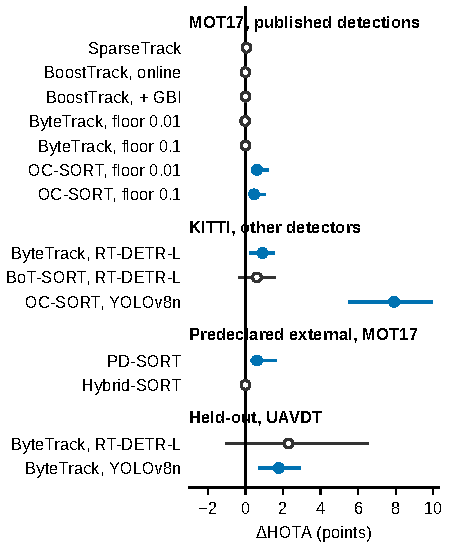
\includegraphics{Fig3.pdf}
\caption{Difference in HOTA, host with \scl{} minus host alone, in points, for every tested cell,
with its 95\% paired-bootstrap interval. Filled circles: interval above zero; open circles:
interval contains zero, or identical output}
\label{fig:forest}
\end{figure}

\subsection{Performance Across Trackers on MOT17}\label{sec:tracker}
Table~\ref{tab:mot17} shows the development trackers on MOT17 val-half. The two-stage trackers with
well-matched detections stayed at the accuracy of their hosts: BoostTrack, online and with GBI, and
ByteTrack at floor 0.1 gave exactly the same output, and ByteTrack at floor 0.01 and SparseTrack
stayed within 0.06 HOTA points, the self-limiting clean mode. The single-stage OC-SORT improved at
both floors (HOTA $+0.61$ and $+0.46$, MOTA $+1.27$ and $+1.26$), with fewer identity switches and
higher HOTA on 7 of 7 sequences, through the continuation rescue.

\begin{table}[!tb]
\caption{Baseline comparison of the development trackers on MOT17 val-half
(published YOLOX-X detections). Paper: number reported by the tracker's
authors. Host: the tracker alone, without \scl{} (our run of the published tracker). $\Delta$: host with
\scl{} minus host, with 95\% paired-bootstrap interval (10,000
resamples, seed 42); bold intervals exclude zero. The floor is the lowest
detector score emitted. IDS: identity switches, a count (lower is better);
--: not reported by the authors.}
\label{tab:mot17}
\centering\footnotesize
\setlength{\tabcolsep}{4pt}
\begin{tabular}{@{}lrrl@{}}
\toprule
Metric & Paper & Host & $\Delta$ [95\% CI]\\
\midrule
\multicolumn{4}{@{}l}{\textit{SparseTrack} \cite{liu2025sparsetrack}}\\
\quad HOTA & 69.2 & 68.88 & $+0.06$ [$-0.01$, $+0.25$]\\
\quad MOTA & 76.8 & 77.85 & $+0.08$ [$-0.03$, $+0.30$]\\
\quad IDF1 & 81.4 & 81.97 & $+0.16$ [$-0.02$, $+0.70$]\\
\quad IDS & -- & 124 & $+7$ [$0$, $+19$]\\
\multicolumn{4}{@{}l}{\textit{BoostTrack, online} \cite{stanojevic2024boosttrack}}\\
\quad HOTA & 68.37 & 68.49 & 0 (identical)\\
\quad MOTA & 75.56 & 75.50 & 0 (identical)\\
\quad IDF1 & 81.35 & 81.41 & 0 (identical)\\
\quad IDS & 118 & 113 & 0 (identical)\\
\multicolumn{4}{@{}l}{\textit{BoostTrack, + GBI} \cite{stanojevic2024boosttrack}}\\
\quad HOTA & 71.33 & 71.72 & 0 (identical)\\
\quad MOTA & 80.55 & 81.03 & 0 (identical)\\
\quad IDF1 & 83.84 & 84.16 & 0 (identical)\\
\quad IDS & 106 & 97 & 0 (identical)\\
\multicolumn{4}{@{}l}{\textit{ByteTrack, floor 0.01} \cite{zhang2022bytetrack}}\\
\quad HOTA & -- & 67.70 & $-0.014$ [$-0.058$, $+0.009$]\\
\quad MOTA & 76.6 & 77.60 & $+0.06$ [$-0.15$, $+0.34$]\\
\quad IDF1 & 79.3 & 79.47 & $-0.031$ [$-0.135$, $+0.035$]\\
\quad IDS & -- & 214 & $+4$ [$-2$, $+13$]\\
\multicolumn{4}{@{}l}{\textit{ByteTrack, floor 0.1} \cite{zhang2022bytetrack}}\\
\quad HOTA & -- & 67.70 & 0 (identical)\\
\quad MOTA & 76.6 & 77.60 & 0 (identical)\\
\quad IDF1 & 79.3 & 79.47 & 0 (identical)\\
\quad IDS & -- & 214 & 0 (identical)\\
\multicolumn{4}{@{}l}{\textit{OC-SORT, floor 0.01} \cite{cao2023ocsort}}\\
\quad HOTA & 66.5 & 66.43 & {\boldmath $+0.61$ [$+0.36$, $+1.24$]}\\
\quad MOTA & 74.9 & 74.67 & {\boldmath $+1.27$ [$+0.17$, $+3.01$]}\\
\quad IDF1 & 77.7 & 78.05 & $+0.66$ [$-0.25$, $+1.60$]\\
\quad IDS & -- & 211 & {\boldmath $-8$ [$-15$, $-2$]}\\
\multicolumn{4}{@{}l}{\textit{OC-SORT, floor 0.1} \cite{cao2023ocsort}}\\
\quad HOTA & 66.5 & 66.44 & {\boldmath $+0.46$ [$+0.27$, $+1.09$]}\\
\quad MOTA & 74.9 & 74.67 & {\boldmath $+1.26$ [$+0.37$, $+3.34$]}\\
\quad IDF1 & 77.7 & 78.05 & {\boldmath $+0.287$ [$+0.003$, $+0.838$]}\\
\quad IDS & -- & 213 & $-14$ [$-38$, $+6$]\\
\bottomrule
\end{tabular}
\end{table}


\subsection{Cross-Detector Evaluation on KITTI}\label{sec:detector}
\begin{figure*}[t]
\centering
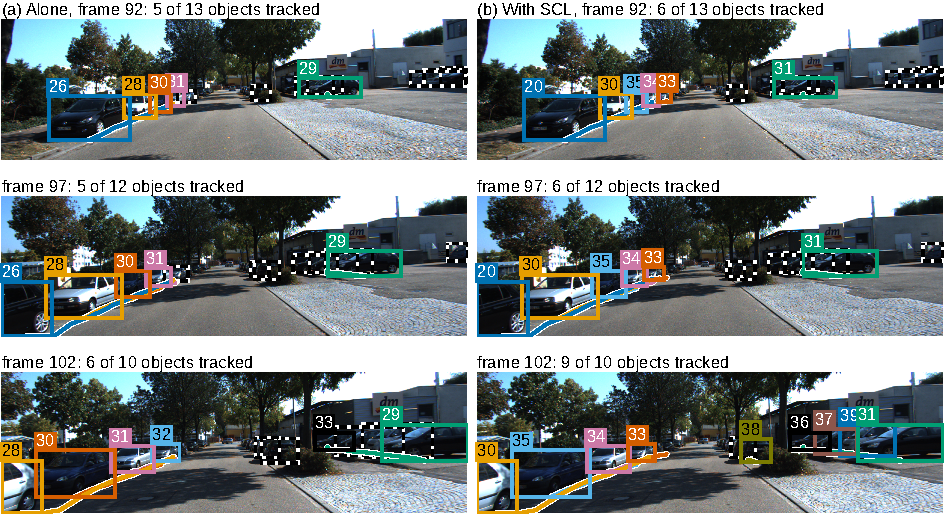
\includegraphics{Fig4.pdf}
\caption{Tracking on KITTI sequence 0001 \cite{geiger2012kitti} with OC-SORT and YOLOv8n, at
frames 92, 97, and 102 (rows): (a) the tracker alone, (b) with \scl{}. Each output track keeps one
ID and one colour over the frames; the line of the same colour is its path over the previous 20
frames (bottom centre of its box). Dashed boxes: labelled objects that no track covers. IDs are
numbered separately in each run. The sequence has the median HOTA gain of the 21 sequences, and
frame 102 is its first frame with the largest gain in tracked objects}
\label{fig:example}
\end{figure*}
Table~\ref{tab:kitti} shows what happens when the detector is replaced. With the noisy RT-DETR-L,
ByteTrack gained 5.98 MOTA, 3.87 IDF1, and 0.91 HOTA points, and BoT-SORT 7.86 MOTA and 3.10 IDF1
points, with 297 and 226 fewer identity switches. With YOLOv8n, OC-SORT gained 7.91 HOTA
points ($[+5.47,+9.98]$), 9.40 MOTA points, and 9.60 IDF1 points; it followed many more objects, as
its missed objects (FN) fell by 5,310, and its identity switches rose with them by 79.
Figure~\ref{fig:example} follows this cell over three frames: each object keeps its ID,
and at frame 102 OC-SORT alone tracked 6 of the 10 labelled objects and with \scl{} 9.

\begin{table}[!tb]
\caption{Baseline comparison under a detector change on KITTI tracking
training (official HOTA, car and pedestrian averaged). Host: the tracker
alone, without \scl{}, with the same detections. $\Delta$: host with \scl{}
minus host, with 95\% paired-bootstrap interval; bold intervals exclude zero.
IDS: identity switches, a count (lower is better). BoT-SORT: KITTI sequence 0020
is left out of both runs, because the BoT-SORT code stopped with a numerical
error in its Kalman update on it; the other 20 sequences are used.}
\label{tab:kitti}
\centering\footnotesize
\setlength{\tabcolsep}{4pt}
\begin{tabular}{@{}lrl@{}}
\toprule
Metric & Host & $\Delta$ [95\% CI]\\
\midrule
\multicolumn{3}{@{}l}{\textit{ByteTrack} \cite{zhang2022bytetrack}\textit{, RT-DETR-L}}\\
\quad HOTA & 50.73 & {\boldmath $+0.91$ [$+0.22$, $+1.55$]}\\
\quad MOTA & 47.27 & {\boldmath $+5.98$ [$+1.16$, $+9.94$]}\\
\quad IDF1 & 64.98 & {\boldmath $+3.87$ [$+1.67$, $+5.06$]}\\
\quad IDS & 686 & {\boldmath $-297$ [$-530$, $-122$]}\\
\multicolumn{3}{@{}l}{\textit{BoT-SORT} \cite{aharon2022botsort}\textit{, RT-DETR-L} (20 sequences)}\\
\quad HOTA & 53.91 & $+0.61$ [$-0.39$, $+1.61$]\\
\quad MOTA & 48.25 & {\boldmath $+7.86$ [$+2.21$, $+13.44$]}\\
\quad IDF1 & 67.74 & {\boldmath $+3.10$ [$+1.00$, $+4.57$]}\\
\quad IDS & 476 & {\boldmath $-226$ [$-369$, $-120$]}\\
\multicolumn{3}{@{}l}{\textit{OC-SORT} \cite{cao2023ocsort}\textit{, YOLOv8n}}\\
\quad HOTA & 36.27 & {\boldmath $+7.91$ [$+5.47$, $+9.98$]}\\
\quad MOTA & 33.99 & {\boldmath $+9.40$ [$+1.10$, $+12.30$]}\\
\quad IDF1 & 50.46 & {\boldmath $+9.60$ [$+5.61$, $+12.16$]}\\
\quad IDS & 91 & {\boldmath $+79$ [$+43$, $+125$]}\\
\bottomrule
\end{tabular}
\end{table}

\begin{table}[!tb]
\caption{Baseline comparison under shifted detector scores on MOT17 val-half. The detector
scores are transformed before the tracker, whose published thresholds stay fixed; $T$ is a logit
temperature, $\sigma(z/T)$. Host: the tracker alone, without \scl{}. $\Delta$: with \scl{} minus host,
with 95\% paired-bootstrap interval (10,000 resamples, seed 42); bold intervals exclude zero.
Emission floor 0.01 (BoostTrack 0.1).}
\label{tab:shift}
\centering\footnotesize
\setlength{\tabcolsep}{4pt}
\begin{tabular}{@{}lrrl@{}}
\toprule
 & \multicolumn{3}{c}{HOTA (\%)}\\
\cmidrule(l){2-4}
Transform & Host & + \scl{} & $\Delta$ [95\% CI]\\
\midrule
\multicolumn{4}{@{}l}{\textit{ByteTrack, official setting} \cite{zhang2022bytetrack}}\\
\quad $s^3$ & 60.92 & 65.81 & {\boldmath $+4.89$ [$+2.60$, $+13.69$]}\\
\quad $0.5\,s$ & 0.00 & 66.17 & {\boldmath $+66.17$ [$+49.32$, $+75.40$]}\\
\quad $T=2$ & 65.84 & 66.95 & {\boldmath $+1.11$ [$+0.35$, $+3.87$]}\\
\quad $T=0.5$ & 67.30 & 67.29 & $-0.009$ [$-0.051$, $+0.005$]\\
\multicolumn{4}{@{}l}{\textit{ByteTrack, library setting} \cite{zhang2022bytetrack}}\\
\quad $s^3$ & 66.31 & 66.31 & $-0.006$ [$-0.384$, $+0.383$]\\
\quad $0.5\,s$ & 66.61 & 66.48 & $-0.14$ [$-0.66$, $+0.14$]\\
\quad $T=2$ & 63.97 & 63.97 & 0 (identical)\\
\quad $T=0.5$ & 66.53 & 66.52 & $-0.006$ [$-0.029$, $+0.001$]\\
\multicolumn{4}{@{}l}{\textit{OC-SORT} \cite{cao2023ocsort}}\\
\quad $s^3$ & 58.34 & 66.60 & {\boldmath $+8.26$ [$+5.86$, $+16.81$]}\\
\quad $0.5\,s$ & 0.00 & 66.72 & {\boldmath $+66.72$ [$+50.32$, $+75.56$]}\\
\quad $T=2$ & 65.99 & 67.22 & {\boldmath $+1.24$ [$+0.52$, $+3.42$]}\\
\quad $T=0.5$ & 66.61 & 67.06 & $+0.45$ [$-0.01$, $+0.97$]\\
\multicolumn{4}{@{}l}{\textit{BoostTrack, online} \cite{stanojevic2024boosttrack}}\\
\quad $s^3$ & 61.33 & 64.84 & {\boldmath $+3.51$ [$+0.85$, $+13.28$]}\\
\quad $T=2$ & 67.59 & 67.59 & 0 (identical)\\
\bottomrule
\end{tabular}
\end{table}

\begin{table}[!tb]
\caption{HOTA (\%) of \scl{} and of two simple adaptive-threshold baselines on KITTI tracking
training (official HOTA, car and pedestrian averaged). Host: the tracker alone, without any layer.
$t_1$, $t_2$: the adaptive baselines, in which the tracker's matching and birth thresholds are set in every frame to the
first or second Otsu split of the logits of the last 10 frames, and the scores are passed unchanged.
Halved: halved detector scores. $\Delta$: \scl{} minus the $t_2$ baseline, with 95\% paired-bootstrap interval below the
value; bold intervals exclude zero.}
\label{tab:baselines}
\centering\footnotesize
\setlength{\tabcolsep}{3pt}
\begin{tabular}{@{}lrrrrc@{}}
\toprule
Cell & Host & $t_1$ & $t_2$ & \scl{} & $\Delta$\\
\midrule
\twol{OC-SORT,}{YOLOv8n} & 36.27 & 39.97 & 41.09 & 44.17 & \cib{+3.09}{+2.00}{+4.03}\\
\addlinespace[3pt]
\begin{tabular}[c]{@{}l@{}}ByteTrack,\\RT-DETR-L,\\halved\end{tabular} & 49.50 & 49.58 & 49.50 & 51.78 & \cib{+2.29}{+0.28}{+4.96}\\
\addlinespace[3pt]
\begin{tabular}[c]{@{}l@{}}OC-SORT,\\YOLOv8n,\\halved\end{tabular} & 0.00 & 37.68 & 43.56 & 46.30 & \cib{+2.74}{+1.32}{+3.34}\\
\bottomrule
\end{tabular}
\end{table}

\begin{table*}[!tp]
\caption{HOTA of ACT \cite{act2026adaptive} and of \scl{} on the same detections, and the
differences \scl{} minus ACT in HOTA and IDF1, with 95\% paired-bootstrap interval below each
value; bold intervals exclude zero. ACT: published parameters, no
tuning. KITTI: official HOTA, car and pedestrian averaged; MOT17: val-half, ACT's own setting;
UAVDT: test split, one vehicle class, ignored regions removed (Sect.~\ref{sec:metrics}).}
\label{tab:act}
\centering\footnotesize
\setlength{\tabcolsep}{5pt}
\begin{tabular}{@{}lllrrcc@{}}
\toprule
Data & Detector & Tracker & ACT & \scl{} & $\Delta$HOTA & $\Delta$IDF1\\
\midrule
KITTI, halved scores & RT-DETR-L & ByteTrack & 49.77 & 51.78 & \cib{+2.01}{+0.01}{+4.76} & \ci{+1.70}{-1.13}{+6.80}\\
KITTI, halved scores & YOLOv8n & OC-SORT & 36.24 & 46.30 & \cib{+10.06}{+6.88}{+12.01} & \cib{+12.03}{+6.85}{+14.69}\\
\addlinespace[4pt]
MOT17, floor 0.01 & YOLOX-X & ByteTrack (official) & 67.46 & 67.68 & \ci{+0.22}{-0.43}{+0.88} & \ci{+0.57}{-0.68}{+2.12}\\
MOT17, floor 0.1 & YOLOX-X & ByteTrack (official) & 67.46 & 67.70 & \ci{+0.23}{-0.40}{+0.90} & \ci{+0.60}{-0.55}{+2.10}\\
\addlinespace[4pt]
UAVDT test & YOLOv8n & ByteTrack & 29.01 & 30.83 & \cib{+1.82}{+0.65}{+3.00} & \cib{+4.00}{+1.85}{+6.22}\\
UAVDT test & RT-DETR-L & ByteTrack & 40.14 & 42.37 & \ci{+2.23}{-0.97}{+6.32} & \ci{+5.35}{-0.03}{+12.47}\\
\bottomrule
\end{tabular}
\end{table*}

\begin{table}[!tb]
\caption{Component ablation and parameter sensitivity of the frozen \scl{} on KITTI (HOTA, \%),
one change at a time, all other values frozen. (a) OC-SORT, YOLOv8n; (b) ByteTrack, RT-DETR-L,
halved scores; (c) OC-SORT, YOLOv8n, halved scores. Below the first row: difference from the
frozen \scl{}, in points.}
\label{tab:compabl}
\centering\footnotesize
\setlength{\tabcolsep}{4pt}
\begin{tabular}{@{}lrrr@{}}
\toprule
Variant & (a) & (b) & (c)\\
\midrule
\scl{} (frozen) & 44.17 & 51.78 & 46.30\\
\addlinespace[2pt]
\multicolumn{4}{@{}l}{\textit{Ablation: one part removed}}\\
No weak detection recovery & $-3.35$ & $+0.06$ & $-1.16$\\
No remap (raw scores) & $0.00$ & $-1.67$ & $-0.61$\\
Always clean (no noisy mode) & $+0.15$ & $-2.40$ & $-2.44$\\
Always noisy (no clean mode) & $+0.08$ & $+0.24$ & $+0.85$\\
No background check & $-0.02$ & $+0.08$ & $+0.15$\\
Overlap-only duplicate rule & $+0.06$ & $+0.13$ & $-0.03$\\
No motion tolerance & $-0.10$ & $-0.04$ & $-0.14$\\
\addlinespace[2pt]
\multicolumn{4}{@{}l}{\textit{Sensitivity: one value changed (frozen value)}}\\
Window $W=5$ (10) & $+0.22$ & $-0.47$ & $-0.48$\\
Window $W=20$ (10) & $+0.56$ & $-0.04$ & $+0.26$\\
Mode median, last 100 frames (all) & $+0.18$ & $-0.19$ & $0.00$\\
Mode median, last 300 frames (all) & $+0.07$ & $+0.12$ & $+0.36$\\
Duplicate and recovery IoU 0.4 (0.5) & $+0.19$ & $+0.16$ & $-0.35$\\
Duplicate and recovery IoU 0.6 (0.5) & $-0.62$ & $-0.34$ & $-0.46$\\
Motion history 50 (100 frames) & $-0.05$ & $+0.06$ & $-0.09$\\
Motion history 200 (100 frames) & $+0.02$ & $+0.08$ & $+0.04$\\
\bottomrule
\end{tabular}
\end{table}

\begin{table}[!tb]
\caption{Baseline comparison on the predeclared external systems (MOT17
val-half, authors' released detections), each evaluated once with the frozen
\scl{}. Paper: number reported by the authors (for PD-SORT, their released
output). Host: the tracker alone, without \scl{} (our run of the published tracker). Reproduction class
against the authors' number (EXACT: $|\Delta\mathrm{HOTA}|\le0.2$; CLOSE:
$\le1.0$ with a documented, untuned cause). $\Delta$: host with \scl{} minus
host, with 95\% paired-bootstrap interval; bold intervals exclude zero. IDS:
identity switches, a count (lower is better); --: not reported.}
\label{tab:external}
\centering\footnotesize
\setlength{\tabcolsep}{4pt}
\begin{tabular}{@{}lrrl@{}}
\toprule
Metric & Paper & Host & $\Delta$ [95\% CI]\\
\midrule
\multicolumn{4}{@{}l}{\textit{PD-SORT} \cite{wang2025pdsort}\textit{, EXACT}}\\
\quad HOTA & 68.01 & 68.01 & {\boldmath $+0.61$ [$+0.27$, $+1.65$]}\\
\quad MOTA & 75.19 & 75.19 & {\boldmath $+1.13$ [$+0.27$, $+3.03$]}\\
\quad IDF1 & 81.03 & 81.03 & {\boldmath $+0.82$ [$+0.43$, $+1.94$]}\\
\quad IDS & -- & 129 & $+2$ [$-9$, $+13$]\\
\multicolumn{4}{@{}l}{\textit{Hybrid-SORT} \cite{yang2024hybridsort}\textit{, CLOSE}}\\
\quad HOTA & 67.1 & 66.70 & 0 (identical)\\
\quad MOTA & 75.8 & 75.52 & 0 (identical)\\
\quad IDF1 & 78.0 & 77.56 & 0 (identical)\\
\quad IDS & -- & 259 & 0 (identical)\\
\bottomrule
\end{tabular}
\end{table}

\begin{table}[!tb]
\caption{Baseline comparison on the held-out UAVDT test split (20 aerial
sequences, not used during design), evaluated once with the frozen \scl{}. Host: ByteTrack alone, without \scl{}, with its published setting. $\Delta$: host
with \scl{} minus host, with 95\% paired-bootstrap interval; bold intervals
exclude zero. IDS: identity switches, a count (lower is better).}
\label{tab:visdrone}
\centering\footnotesize
\setlength{\tabcolsep}{4pt}
\begin{tabular}{@{}lrl@{}}
\toprule
Metric & Host & $\Delta$ [95\% CI]\\
\midrule
\multicolumn{3}{@{}l}{\textit{ByteTrack, RT-DETR-L} \cite{zhang2022bytetrack,zhao2024rtdetr}}\\
\quad HOTA & 40.07 & $+2.30$ [$-1.05$, $+6.55$]\\
\quad MOTA & 3.29 & {\boldmath $+24.70$ [$+10.06$, $+51.08$]}\\
\quad IDF1 & 48.59 & {\boldmath $+5.74$ [$+0.13$, $+13.11$]}\\
\quad IDS & 1041 & {\boldmath $-586$ [$-951$, $-248$]}\\
\multicolumn{3}{@{}l}{\textit{ByteTrack, YOLOv8n} \cite{zhang2022bytetrack,jocher2023yolov8}}\\
\quad HOTA & 29.05 & {\boldmath $+1.77$ [$+0.70$, $+2.94$]}\\
\quad MOTA & 16.27 & $+1.02$ [$-1.06$, $+2.86$]\\
\quad IDF1 & 34.52 & {\boldmath $+3.97$ [$+1.88$, $+6.17$]}\\
\quad IDS & 719 & {\boldmath $-326$ [$-691$, $-73$]}\\
\bottomrule
\end{tabular}
\end{table}


\subsection{Robustness to Detection Score Shifts}\label{sec:shift}
Table~\ref{tab:shift} shows the trackers under the four score transforms. Halving the scores
reduced ByteTrack (official setting) and OC-SORT to 0 HOTA; with the layer they reached 66.17 and
66.72. Cubing reduced them to 60.92 and 58.34, and the layer restored them to 65.81 and 66.60;
BoostTrack rose from 61.33 to 64.84. With $T=2$, the layer raised ByteTrack and OC-SORT by 1.11 and
1.24 points. The library setting of ByteTrack, whose low thresholds already accept the changed
scores, stayed within 0.14 points. Over the 14 conditions, the layer raised HOTA significantly in 7
and lowered it significantly in none.


\subsection{Comparison with Adaptive Thresholding Methods}\label{sec:baselines}
Two simple baselines set the tracker's matching and birth thresholds in every frame to the first or
second Otsu split of the logits of the last 10 frames, $t_1$ or $t_2$, and pass the scores
unchanged. On KITTI (Table~\ref{tab:baselines}), \scl{} reached the highest HOTA in all three
cells, 2.2 to 8.6 points above the baselines, with intervals against the $t_2$ baseline above zero
in every cell, so adaptive thresholds alone do not explain the gains. With OC-SORT, \scl{} also had
fewer identity switches than both baselines (170 against 1,545 and 250 with YOLOv8n; 308 against
1,975 and 492 under halved scores).

\emph{Logit-to-score conversion.} The baselines and \scl{} find their splits on logits, while a
tracker compares its thresholds with scores, so a split must be converted back with the logistic
function: the baselines pass $\sigma(t_1)$ or $\sigma(t_2)$ to the tracker, and \scl{} passes
$\min(a,\sigma(t_2))$ in clean frames (Eq.~\eqref{eq:clean}) and 0.5 with remapped scores in noisy
frames. The thresholds recorded in every frame matched these values exactly, with zero difference,
in every frame with a split of all eight baseline runs (7,987 frames with RT-DETR-L and 7,940
with YOLOv8n per run) and in all clean and noisy frames of \scl{} in the four KITTI cells. The baselines therefore received the thresholds they were meant to have.

\emph{ACT.} ACT \cite{act2026adaptive} is the closest published method: in every frame it sets
ByteTrack's high and low thresholds from the first quartile and the number of the current scores,
choosing between preset levels. It works on the scores directly, so it needs no conversion, and
under halved scores it receives the halved scores, as \scl{} does. It was run with its published
parameters, without retuning, on the same detections and hosts as \scl{} (Table~\ref{tab:act}):
its high threshold became the host's matching threshold and its low threshold the lower bound of
the second step, while the host's birth threshold and matching tolerance stayed unchanged; with
OC-SORT, which has one threshold, the high threshold served as that threshold. Before the
comparison, the ACT runner was run with the host's own thresholds and reproduced the output of the
host alone exactly in all 84 KITTI, 14 MOT17, and 40 UAVDT sequence runs. \scl{} reached higher HOTA
than ACT in every row, significantly under halved
scores ($+2.01$ and $+10.06$ points) and with YOLOv8n on UAVDT ($+1.82$), and also in the MOT17
setting for which ACT was designed. With RT-DETR-L on UAVDT, \scl{} reached a MOTA of 27.99 against
5.34 ($+22.65$, $[+9.03,+47.21]$), because the fixed score levels of ACT removed few of the host's
false positives (178,219 against 78,975). \scl{} also had fewer identity switches than ACT on
MOT17 and UAVDT (up to 418 fewer). In no tested cell, including the two KITTI cells with the
original scores, was the HOTA of \scl{} significantly below that of ACT.

\subsection{Component Ablation and Parameter Sensitivity}\label{sec:ablation}
Table~\ref{tab:compabl} removes one part of the frozen \scl{}, or changes one of its values, at a
time on the three KITTI cells of Table~\ref{tab:baselines}, with the same detections and trackers.
Each part matters where its step acts. Without the weak detection recovery, the single-stage
OC-SORT lost 3.35 and 1.16 HOTA points, as it has no low-score step of its own. Without the noisy
mode (always clean), the halved-score cells lost 2.40 and 2.44 points, and without the remap up to
1.67 points. Always acting in the noisy mode stayed within 0.85 points of \scl{} on these KITTI
streams, which are noisy in most of their frames; on well-matched MOT17 trackers, however, always
acting is the earlier design \aob{}, which lowered HOTA by 4.15 to 5.89 points
(Table~\ref{tab:prior}). The mode decision is thus what lets one configuration serve both kinds of
stream. The background check, the duplicate rule, and the motion tolerance changed HOTA by at most
0.15 points on KITTI.

The sensitivity analysis, planned before the runs, changed the window $W$, the frames whose median
decides the mode, the IoU of the duplicate and recovery rules, and the motion history. For every
value and cell, HOTA stayed within 0.62 points of the frozen \scl{}, and within 0.24 points on the
fourth KITTI cell, ByteTrack with the original RT-DETR-L scores. The frozen values lie on a flat
part of the response, so none of them needs tuning for these detectors and trackers. The shorter
median windows, which bound the delay of the mode (Sect.~\ref{sec:regimes}), changed HOTA by at most
0.36 points on these streams.


\subsection{Generalization to Unseen Trackers}\label{sec:external}
Table~\ref{tab:external} gives the two predeclared external systems. PD-SORT \cite{wang2025pdsort}
was reproduced exactly. With \scl{}, its HOTA rose by 0.61 points ($[+0.27,+1.65]$), its MOTA by
1.13 ($[+0.27,+3.03]$), and its IDF1 by 0.82 ($[+0.43,+1.94]$), with higher HOTA on 7 of 7
sequences; like OC-SORT, it is a single-stage tracker, but it was not seen during design.
Hybrid-SORT \cite{yang2024hybridsort}, a two-stage tracker, gave identical output, as predicted
before the run.


\subsection{Cross-Dataset Generalization on UAVDT}\label{sec:visdrone}
On the held-out UAVDT test split (Table~\ref{tab:visdrone}), \scl{} raised the HOTA of the YOLOv8n
stream by 1.77 points ($[+0.70,+2.94]$) and its IDF1 by 3.97 points, and cut identity switches by
45\%. With RT-DETR-L, whose host produced many false positives (MOTA 3.29), \scl{} raised MOTA by
24.70 points ($[+10.06,+51.08]$) and IDF1 by 5.74 points, and cut false positives by 58\% and
identity switches by 56\%. No HOTA decrease was detected with either detector.


\section{Discussion and Practical Implications}\label{sec:discussion}

\emph{The score scale is part of the MOT system.} Halving the scores reduced ByteTrack and OC-SORT
from 67.70 and 66.43 HOTA to 0, and with RT-DETR-L on UAVDT ByteTrack reached a MOTA of only 3.29.
The fixed thresholds of a tracker hold only for the detector they were tuned for, so the score
scale deserves the same attention as the association method.

\emph{Self-limiting by design.} In the clean mode the layer keeps the tracker's thresholds and
scores, so a well-matched tracker receives its normal input; \aob{}, which always intervened,
lowered the same trackers by 4.15 to 5.89 HOTA points. Single-stage trackers gain through the
recovery of weak detections, and two-stage trackers when the detector is noisy.

\emph{Deployment.} \scl{} needs no training, no GPU, and no access to the inside of the detector or
the tracker. On a CPU it takes 2.95 ms per frame, small next to the 42 ms of the detector, and the
tracker itself ran faster with it (1.43 against 2.04 ms per frame); the end-to-end time rose by
only 4.5\% (4-vCPU Intel Xeon at 2.10 GHz, no GPU, YOLOv8n and ByteTrack on three KITTI sequences,
2,279 timed frames). A new tracker is added through its four published contract
values and an adapter, without changes to the rules. Because the mode and the confident share
$\rho$ need no labels, they can also be logged as a running check of whether a new or retrained
detector still fits the tracker it feeds.

\emph{Operational assumptions.} The layer relies on five conditions. (i) The detector's score
orders its candidates by confidence; the splits move exactly with a stretch or shift of the
logits, and approximately with other order-preserving changes such as cubing, under which the
layer still restored the trackers (Sect.~\ref{sec:shift}). (ii) Clutter gives more candidates
than objects do; when it does not, the background check treats the window as clean. (iii) The
classes of one detector share a score scale, as the splits pool the scores of all classes. (iv)
The tracker uses score thresholds that an adapter can set before each update, and its four
contract values are published. (v) The camera-motion cue measures a global image shift, so it
reflects the motion of the camera rather than that of single objects.

\emph{Limitations.} The mode is a property of the whole stream, so after a lasting change of the
detector within one stream the rescoring of the noisy mode follows with a delay
(Sect.~\ref{sec:regimes}); the splits and the clean-mode thresholds adapt within 10 frames. The
rules and their values are fixed, not learned; the sensitivity analysis found HOTA within 0.62
points for the tested values, but other values, such as the mode threshold of one half, were not
varied. The evaluation covers seven trackers, four detection sources, and three datasets of people
and vehicles; other object types, other detector families, and trackers without score thresholds,
such as end-to-end trackers, were not tested, and the running time was measured on one processor
type. These limits define the next tests rather than changes to the frozen layer.

\section{Conclusion}\label{sec:conclusion}

This paper treated the compatibility between a detector's score scale and a tracker's thresholds
as a property that can be checked and restored online, without labels and without changing either
component. \scl{} checks it with nested Otsu splits of recent logits and a whole-stream majority
rule, leaves compatible pairs as they are, and restores incompatible ones through the tracker's own
published settings: it chooses and rescores the candidates, sets the thresholds, and recovers weak
detections that continue tracks. The frozen layer demonstrated this compatibility on seven trackers
and four detection sources: it restored two trackers from 0 to about 66 HOTA under halved scores,
improved both single-stage trackers on every MOT17 sequence, raised MOTA by up to 24.70 points with
a mismatched detector on held-out aerial data, kept well-matched trackers at their own accuracy
with no statistically detected HOTA loss, reached higher HOTA than simple adaptive thresholds and
ACT, stayed within 0.62 HOTA points under changes of its values, and took 2.95 ms per frame on a
CPU. Detector--tracker compatibility can therefore be managed as part of the tracking system, so a
detector can be replaced or retrained without retuning the tracker. Future work will test the layer
with more detector families, object types, and trackers.


\FloatBarrier
\backmatter

\bibliography{references}

\end{document}
